\chapter{O Sistema Test-Manager}

Este capítulo apresenta o sistema Test-Manager implementado, detalhando a materialização prática da arquitetura planejada, o controle de acesso hierárquico por perfis e as interfaces gráficas que atendem aos requisitos funcionais e casos de uso especificados no Capítulo 4.

\section{Arquitetura da Solução e Controle de Acesso}

A solução adota uma arquitetura web monolítica estruturada sob o padrão \textit{Model-View-Controller} (MVC), implementada por meio do framework Laravel (PHP) em conjunto com o banco de dados relacional MySQL. No lado do servidor, os controladores (\textit{Controllers}) concentram as regras de negócio, a validação de formulários e a orquestração do versionamento de testes, enquanto a camada de persistência utiliza o mapeamento objeto-relacional Eloquent ORM para garantir a integridade referencial das transações. Na camada de apresentação (\textit{View}), o motor de templates Blade renderiza interfaces dinâmicas e responsivas estilizadas com o framework Bootstrap 5 (RNF01). Toda a infraestrutura executa de forma isolada em contêineres Docker, assegurando padronização entre os ambientes de desenvolvimento e implantação.

O controle de acesso e a segurança da plataforma (RF01, RF02 e RNF02) apoiam-se no mecanismo nativo de sessões autenticadas do Laravel, com senhas criptografadas via algoritmo BCrypt e proteção contra falsificação de requisições (\textit{CSRF Token}). A autorização operacional ocorre em duas frentes complementares:
\begin{itemize}
    \item \textbf{Restrição na camada de apresentação:} As diretivas condicionais do Blade ocultam botões de ação, menus e formulários não autorizados para o papel do usuário logado, adaptando a interface ao escopo de cada ator;
    \item \textbf{Validação estrita no servidor:} Os controladores e \textit{middlewares} verificam o atributo de perfil (\texttt{role}) e o vínculo do usuário com o projeto antes de processar qualquer requisição HTTP, bloqueando acessos diretos não autorizados via URL.
\end{itemize}

Dessa forma, o perfil \textbf{Coordenador} detém visibilidade administrativa sobre seus projetos, equipes, roteiros de teste e métricas; o \textbf{Tester} visualiza e executa exclusivamente os casos de teste e versões atribuídos à sua responsabilidade; e o \textbf{Desenvolvedor} acessa e atualiza estritamente os defeitos (\textit{bugs}) sob sua incumbência técnica.

\section{Interfaces e Fluxos Operacionais do Sistema}

O painel administrativo do Test-Manager materializa os módulos modelados no Capítulo 4. Para cada funcionalidade apresentada a seguir, descreve-se o fluxo operacional na perspectiva do usuário, relacionando os elementos visuais da tela às regras de negócio e aos requisitos funcionais correspondentes. O Quadro \ref{quad:modulos_sistema} sintetiza os módulos implementados e os perfis autorizados em cada etapa do fluxo de qualidade.

\begin{quadro}[!htb]
\centering
\caption{Módulos do sistema Test-Manager, funcionalidades e perfis de acesso.}
\label{quad:modulos_sistema}
\small
\begin{tabularx}{\textwidth}{|p{2.5cm}|X|p{3.4cm}|p{2.2cm}|}
\hline
\textbf{Módulo} & \textbf{Principais Funcionalidades} & \textbf{Perfis Autorizados} & \textbf{Requisitos} \\ \hline
Acesso & Autenticação de usuários, proteção de sessão e cadastro inicial de coordenador. & Todos os perfis & RF01, RF02 \\ \hline
Dashboard & Exibição de indicadores de testes (aprovados, reprovados, pendentes), defeitos por severidade e exportação de relatório em PDF. & Coordenador, Tester e Desenvolvedor & RF12 \\ \hline
Projetos e Equipe & Cadastro e gestão de projetos de software, cadastro de usuários e alocação de membros ($N:N$). & Coordenador & RF03, RF04 \\ \hline
Casos de Teste & Criação manual, importação em lote via arquivo \texttt{.csv}, versionamento automático e atribuição de Testers. & Coordenador (gestão) e Tester (consulta) & RF05, RF06, RF07, RF08 \\ \hline
Execução e Avaliação & Execução passo a passo do roteiro de teste, aprovação ou reprovação de versão com geração automática de nova versão. & Tester e Coordenador & RF07, RF09, RF13 \\ \hline
Defeitos (\textit{Bugs}) & Registro obrigatório de defeito na reprovação (com upload de \textit{print}), atribuição de desenvolvedor e atualização de status de correção. & Tester/Coordenador (registro) e Desenvolvedor (correção) & RF10, RF11, RF13 \\ \hline
\end{tabularx}
\fonte{Elaborado pelo autor (2026).}
\end{quadro}

\subsection{Acesso ao Sistema e Painel de Indicadores (Dashboard)}

\subsubsection{Login e Autenticação}

O acesso inicial ao Test-Manager materializa os requisitos RF01 e RF02 e o caso de uso UC01. Na tela de autenticação (Figura \ref{fig:tela_login}), o usuário informa seu endereço de e-mail institucional e senha. Caso as credenciais sejam válidas e o cadastro esteja ativo no banco de dados, o sistema inicia a sessão autenticada e redireciona o integrante diretamente ao painel principal configurado para o seu perfil de acesso.

\begin{figure}[H]
    \centering
    \caption{Tela de login e autenticação do Test-Manager.}
    \label{fig:tela_login}
    \vspace{0.2cm}
    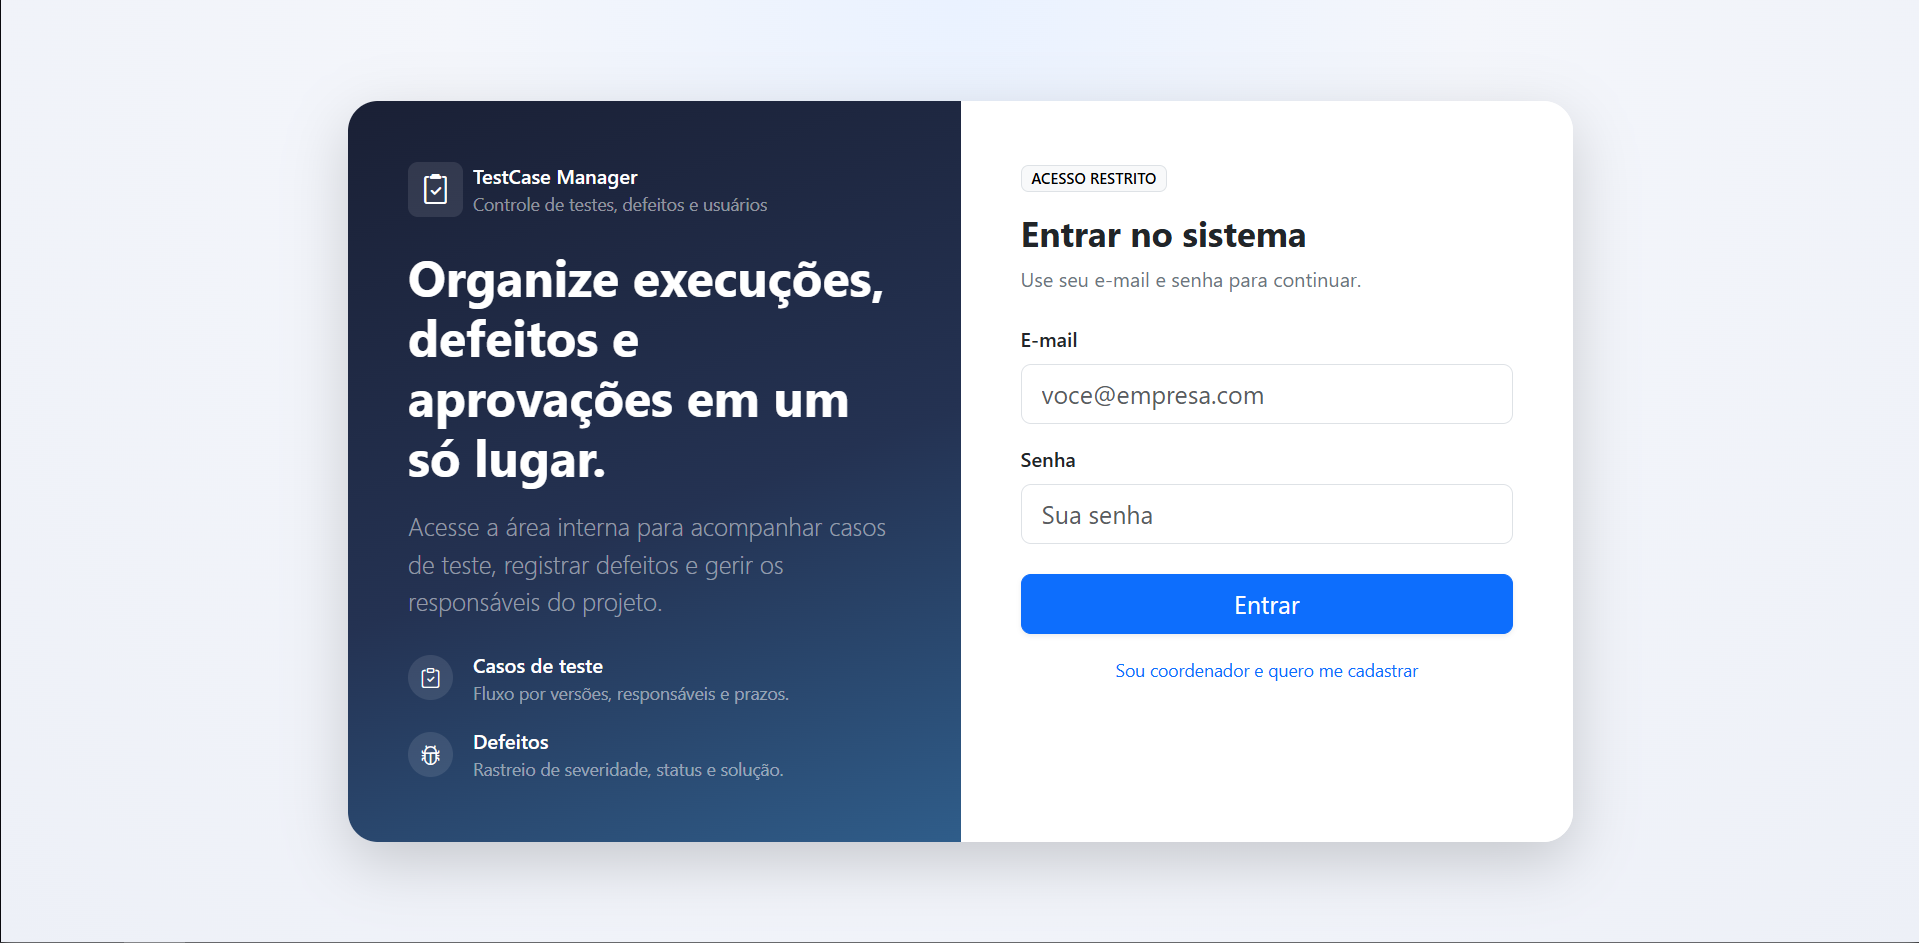
\includegraphics[width=0.85\textwidth, height=0.75\textheight, keepaspectratio]{./figuras/tela_login.png} \\
    \vspace{0.2cm}
    {\raggedright \small Fonte: Elaborado pelo autor (2026).\par}
\end{figure}

\subsubsection{Dashboard Gerencial e Relatórios}

Após a autenticação, o usuário visualiza o \textit{Dashboard} da plataforma (Figura \ref{fig:tela_dashboard}), que atende ao requisito RF12. Para o perfil Coordenador, o painel consolida em tempo real as métricas de qualidade dos projetos sob sua gestão, exibindo cartões totalizadores com o volume de projetos ativos, o total de casos de teste cadastrados, a proporção de versões aprovadas, pendentes e reprovadas, bem como a distribuição de defeitos abertos e resolvidos. Adicionalmente, o coordenador dispõe da funcionalidade de exportação consolidada em formato PDF (UC03), permitindo documentar o estado de estabilidade do software avaliado para fins acadêmicos e gerenciais.

\begin{figure}[H]
    \centering
    \caption{Painel de indicadores (Dashboard) do Test-Manager.}
    \label{fig:tela_dashboard}
    \vspace{0.2cm}
    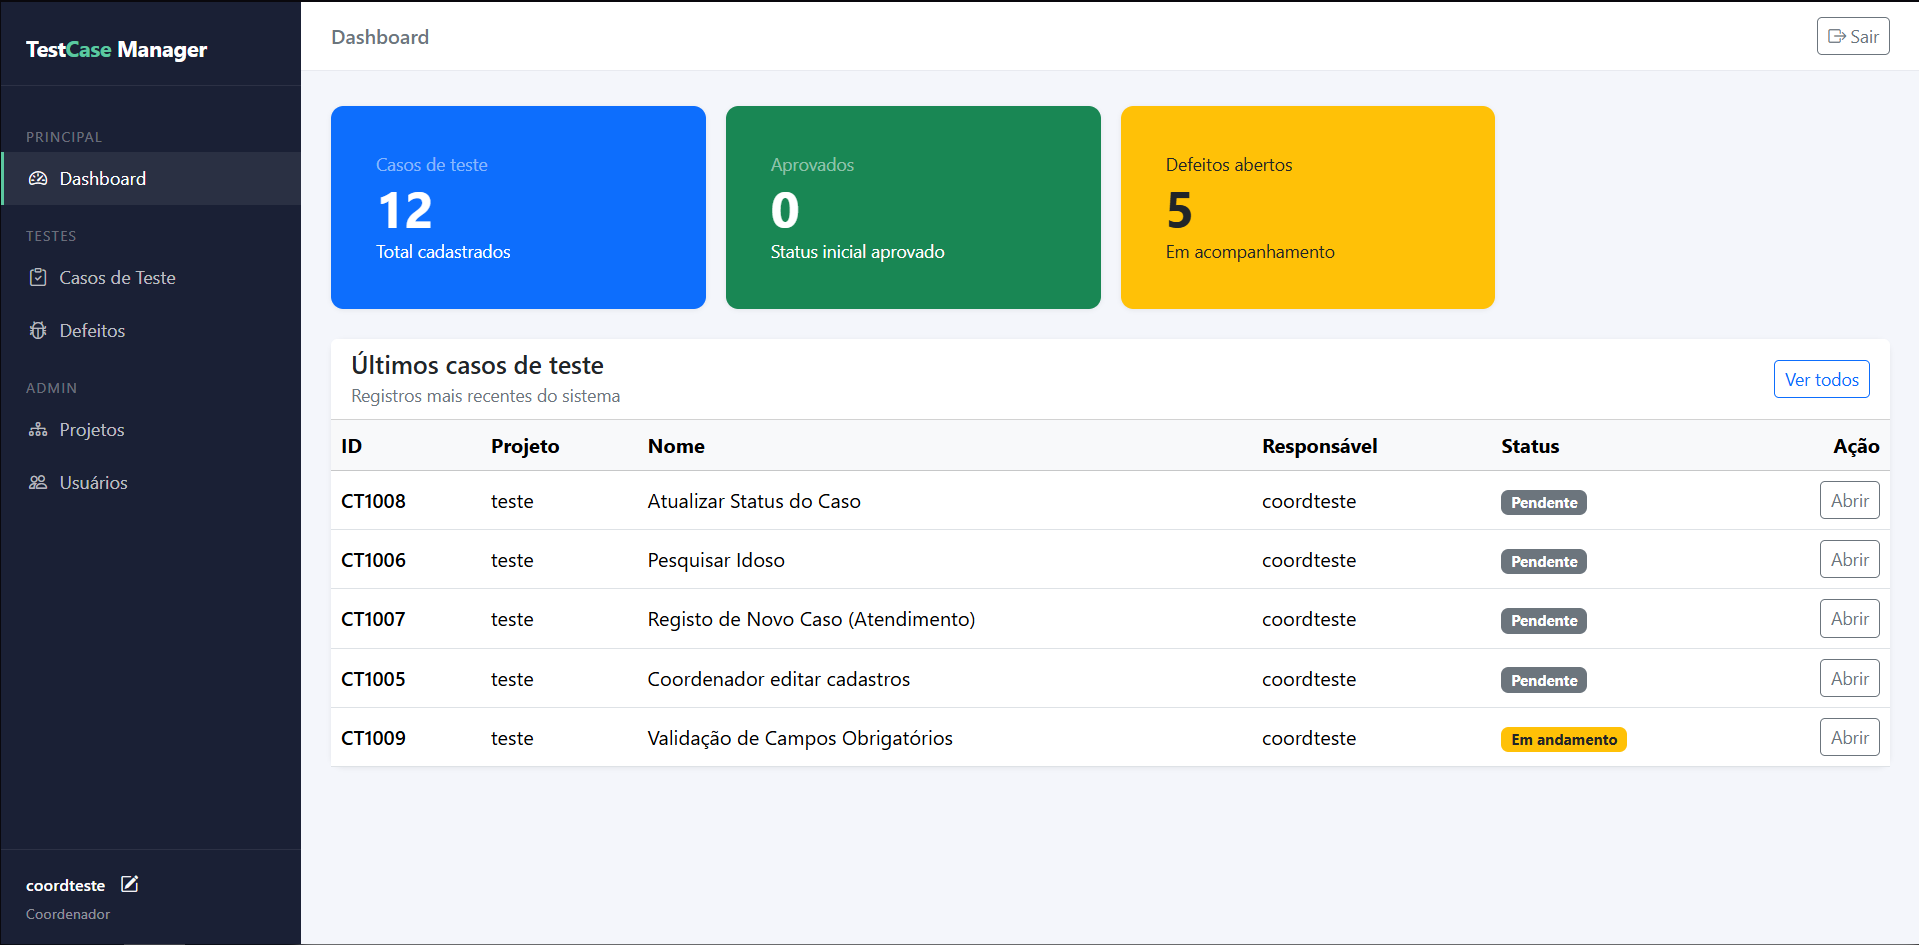
\includegraphics[width=0.92\textwidth, height=0.75\textheight, keepaspectratio]{./figuras/tela_dashboard.png} \\
    \vspace{0.2cm}
    {\raggedright \small Fonte: Elaborado pelo autor (2026).\par}
\end{figure}

\subsection{Gestão de Projetos, Equipes e Casos de Teste}

\subsubsection{Cadastro de Projetos e Alocação de Usuários}

Este módulo implementa os requisitos RF03 e RF04 (casos de uso UC02 e UC04). Na interface de gestão de projetos (Figura \ref{fig:tela_projetos}), o Coordenador registra os sistemas em desenvolvimento no campus, especificando nome, descrição, objetivos, escopo e critérios formais de entrada e saída. Na mesma estrutura, o coordenador cadastra novos usuários com os papéis de Tester ou Desenvolvedor e realiza a vinculação desses integrantes aos projetos correspondentes, garantindo que cada membro visualize apenas os artefatos das equipes em que está alocado.

\begin{figure}[H]
    \centering
    \caption{Tela de gestão de projetos e vinculação de equipe.}
    \label{fig:tela_projetos}
    \vspace{0.2cm}
    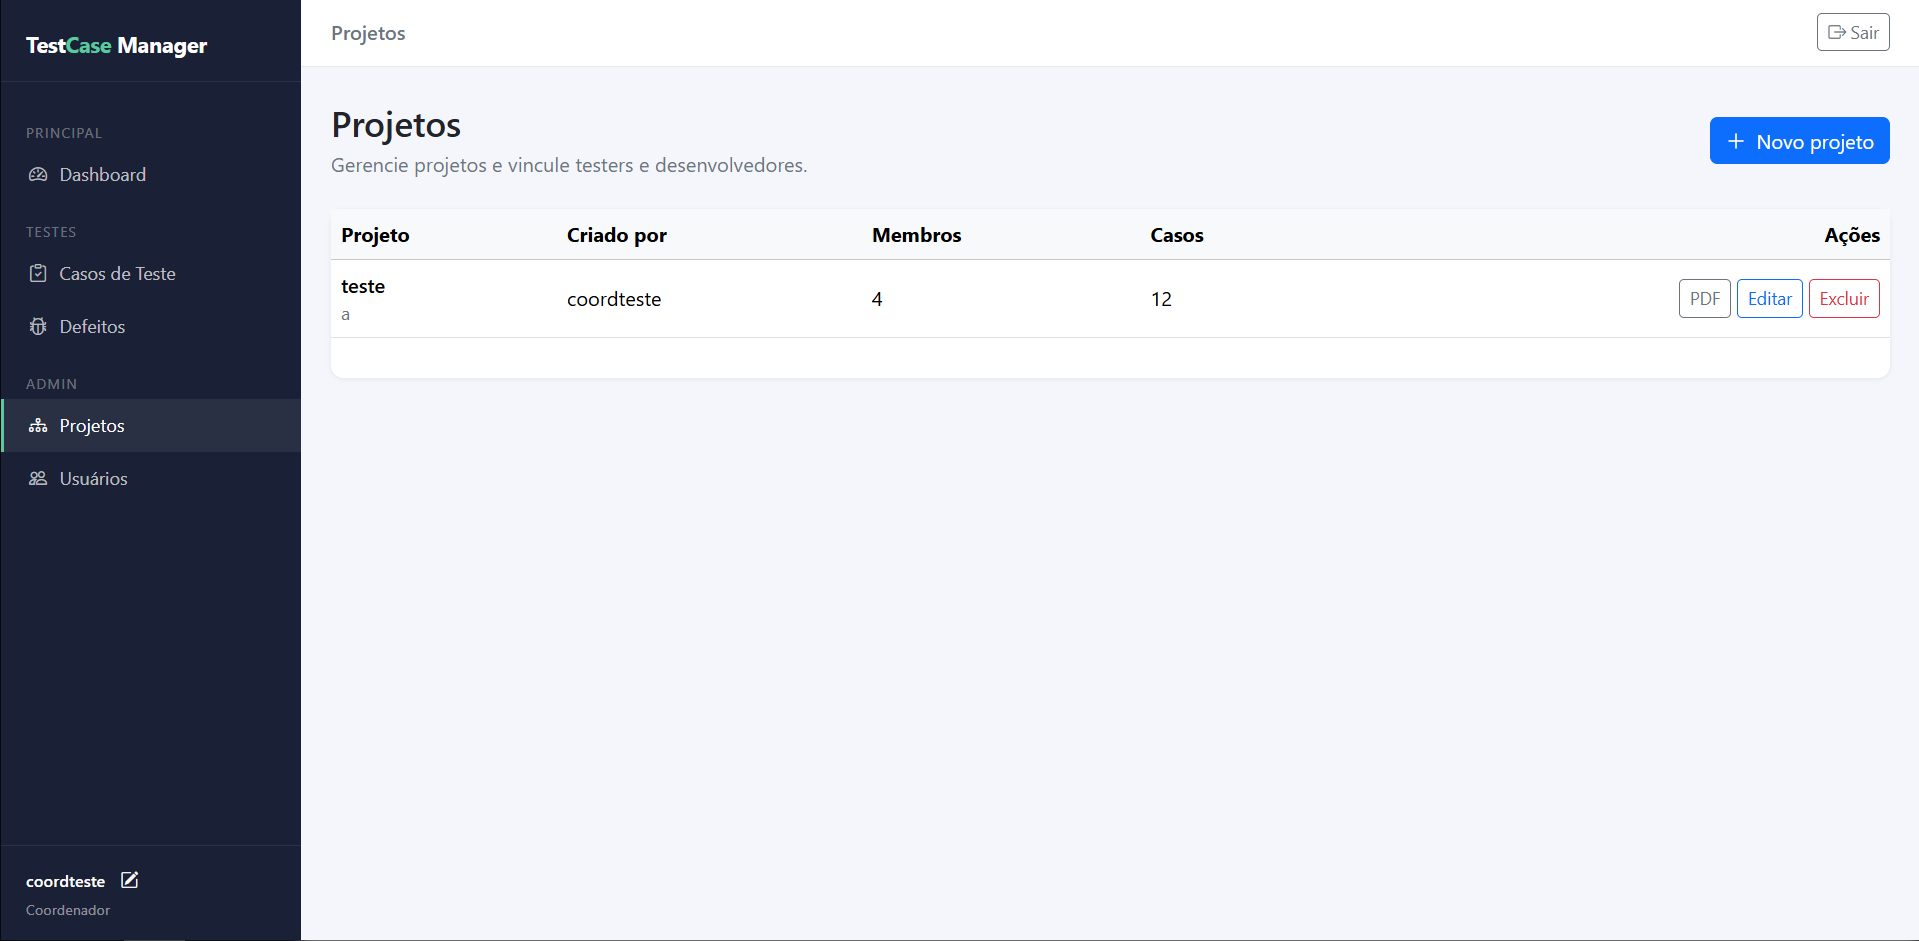
\includegraphics[width=0.92\textwidth, height=0.75\textheight, keepaspectratio]{./figuras/tela_projetos.png} \\
    \vspace{0.2cm}
    {\raggedright \small Fonte: Elaborado pelo autor (2026).\par}
\end{figure}

\subsubsection{Gestão de Casos de Teste e Importação em Lote}

A estruturação dos roteiros de validação contempla os requisitos RF05, RF06, RF07 e RF08 (UC05). Na tela de listagem e criação de casos de teste (Figura \ref{fig:tela_casos}), o Coordenador pode cadastrar cenários individualmente --- definindo título, descrição, pré-condições, passos sequenciais de execução, resultado esperado, prazo e Tester responsável --- ou utilizar a ferramenta de importação em lote mediante o envio de arquivos estruturados no formato \texttt{.csv}. Ao registrar um novo caso de teste, o sistema gera automaticamente um código identificador padronizado (como \texttt{CT-001}) e instancia sua versão inicial (\texttt{v1.0}) com status \textit{Pendente}, implementando paginação nas listagens (RNF03) para preservar a fluidez da navegação.

\begin{figure}[H]
    \centering
    \caption{Listagem e gerenciamento de casos de teste no painel.}
    \label{fig:tela_casos}
    \vspace{0.2cm}
    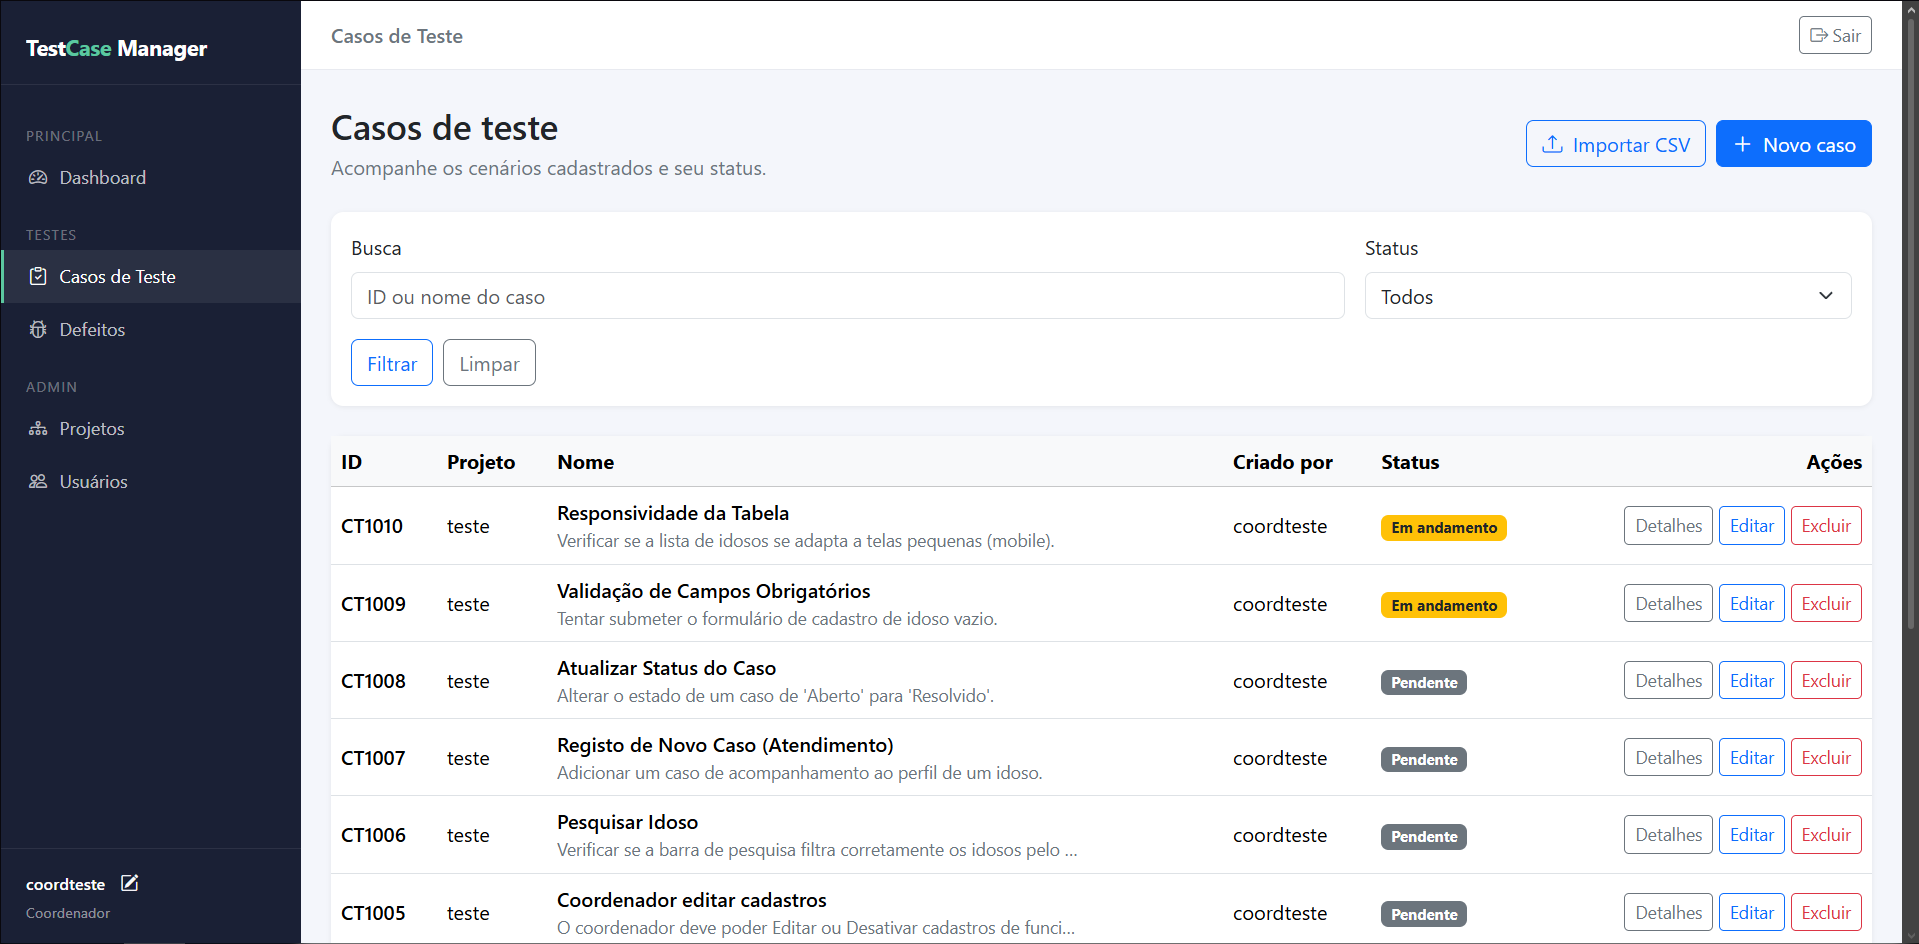
\includegraphics[width=0.92\textwidth, height=0.75\textheight, keepaspectratio]{./figuras/tela_casos.png} \\
    \vspace{0.2cm}
    {\raggedright \small Fonte: Elaborado pelo autor (2026).\par}
\end{figure}

\subsection{Execução de Testes, Rastreamento de Defeitos e Auditoria}

\subsubsection{Execução de Casos de Teste e Versionamento Automático}

O módulo de avaliação operacionaliza os requisitos RF07, RF09 e RF13 (casos de uso UC06, UC07 e UC08). Ao acessar os detalhes de um caso de teste atribuído ao seu perfil (Figura \ref{fig:tela_execucao_caso}), o Tester inspeciona as pré-condições, os passos de reprodução e o resultado esperado da versão ativa. Caso o software avaliado se comporte conforme especificado, o Tester aprova a versão, encerrando o ciclo de validação daquele cenário. Por outro lado, caso seja constatada uma falha durante a execução, o acionamento da reprovação retém a avaliação em sessão e direciona o usuário obrigatoriamente ao formulário de registro de defeito. Concluído o relato da falha, o sistema consolida a versão atual como \textit{Reprovada}, cria automaticamente a versão subsequente (\texttt{v2.0}, \texttt{v3.0}) com status \textit{Pendente} para reteste futuro e grava o evento na linha do tempo de auditoria (\texttt{Historico}) exibida na própria tela.

\begin{figure}[H]
    \centering
    \caption{Tela de detalhes do caso de teste, avaliação de versões e histórico de auditoria.}
    \label{fig:tela_execucao_caso}
    \vspace{0.2cm}
    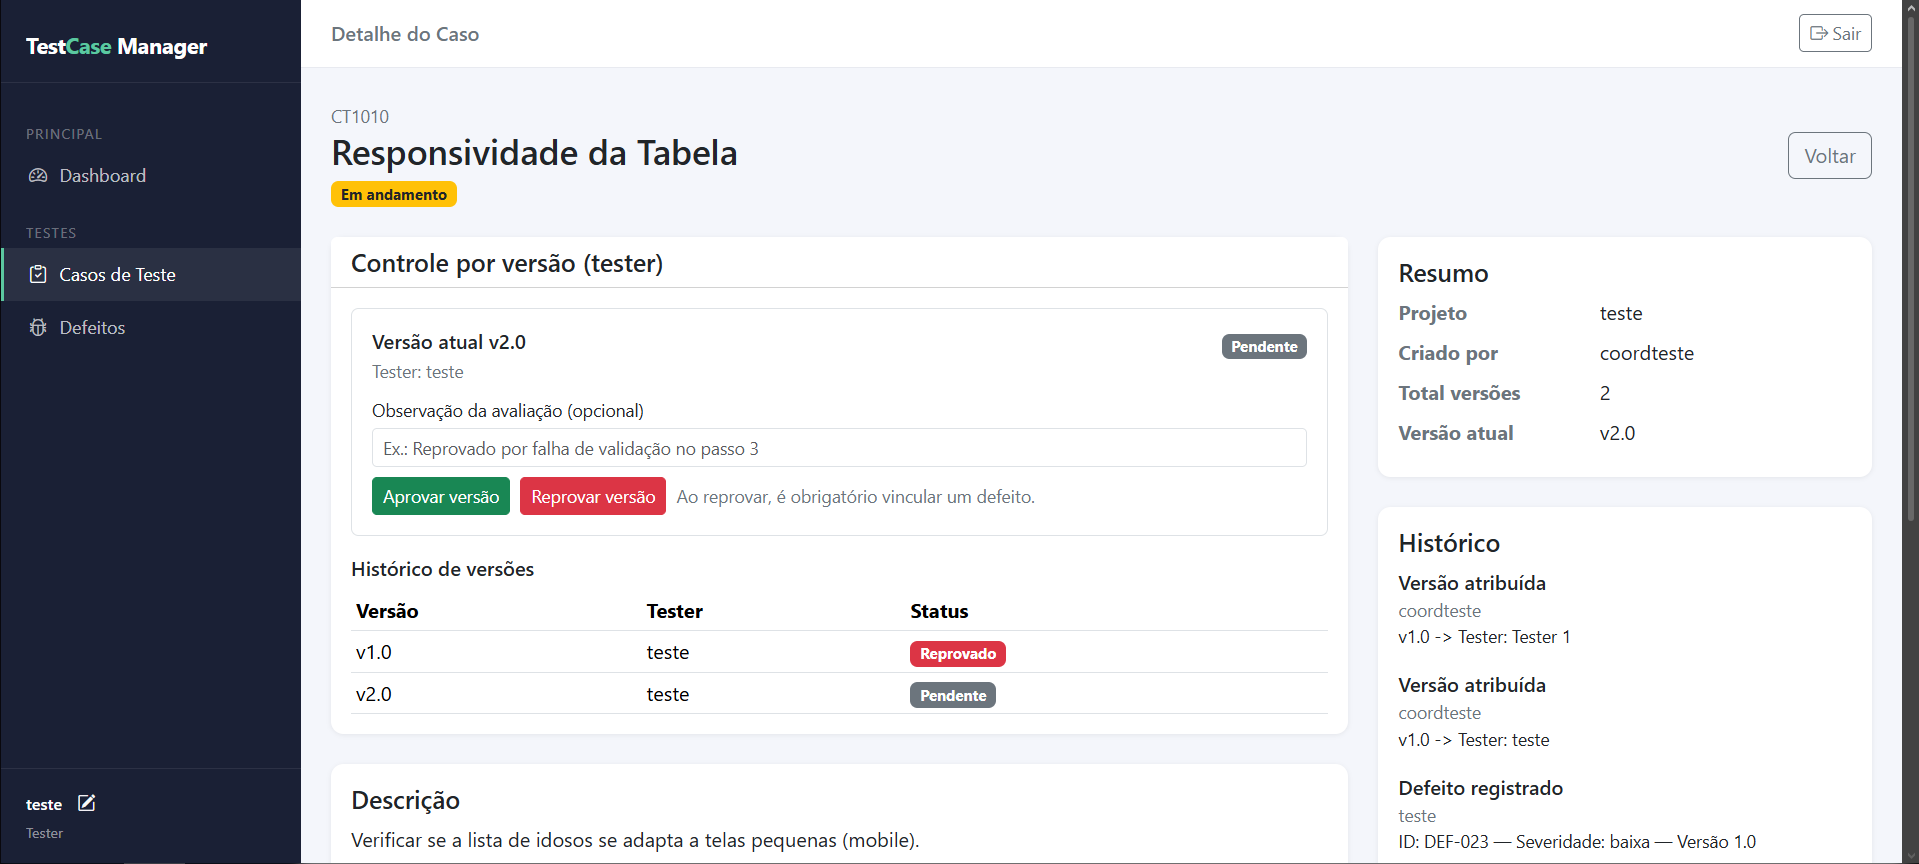
\includegraphics[width=0.92\textwidth, height=0.75\textheight, keepaspectratio]{./figuras/tela_execucao_caso.png} \\
    \vspace{0.2cm}
    {\raggedright \small Fonte: Elaborado pelo autor (2026).\par}
\end{figure}

\subsubsection{Registro e Ciclo de Vida de Defeitos (Bugs)}

O gerenciamento de falhas atende aos requisitos RF10, RF11 e RF13 (casos de uso UC09, UC10 e UC11). Na tela de registro e acompanhamento de defeitos (Figura \ref{fig:tela_defeitos}), o relator documenta a anomalia informando a versão do teste afetada, a descrição detalhada do problema, os passos exatos para reprodução, o grau de severidade (\textit{Baixa}, \textit{Média} ou \textit{Alta}) e anexa a captura de tela (\textit{print}) que evidencia o erro visualmente. O Coordenador designa o Desenvolvedor responsável e estipula o prazo de solução. Na visão do Desenvolvedor, o painel lista todos os defeitos sob sua responsabilidade, permitindo consultar os passos e evidências anexadas e atualizar o status do registro para \textit{Resolvido} assim que a correção do código-fonte é finalizada, notificando a rastreabilidade no histórico do caso de teste correspondente.

\begin{figure}[H]
    \centering
    \caption{Módulo de registro e acompanhamento do ciclo de vida de defeitos.}
    \label{fig:tela_defeitos}
    \vspace{0.2cm}
    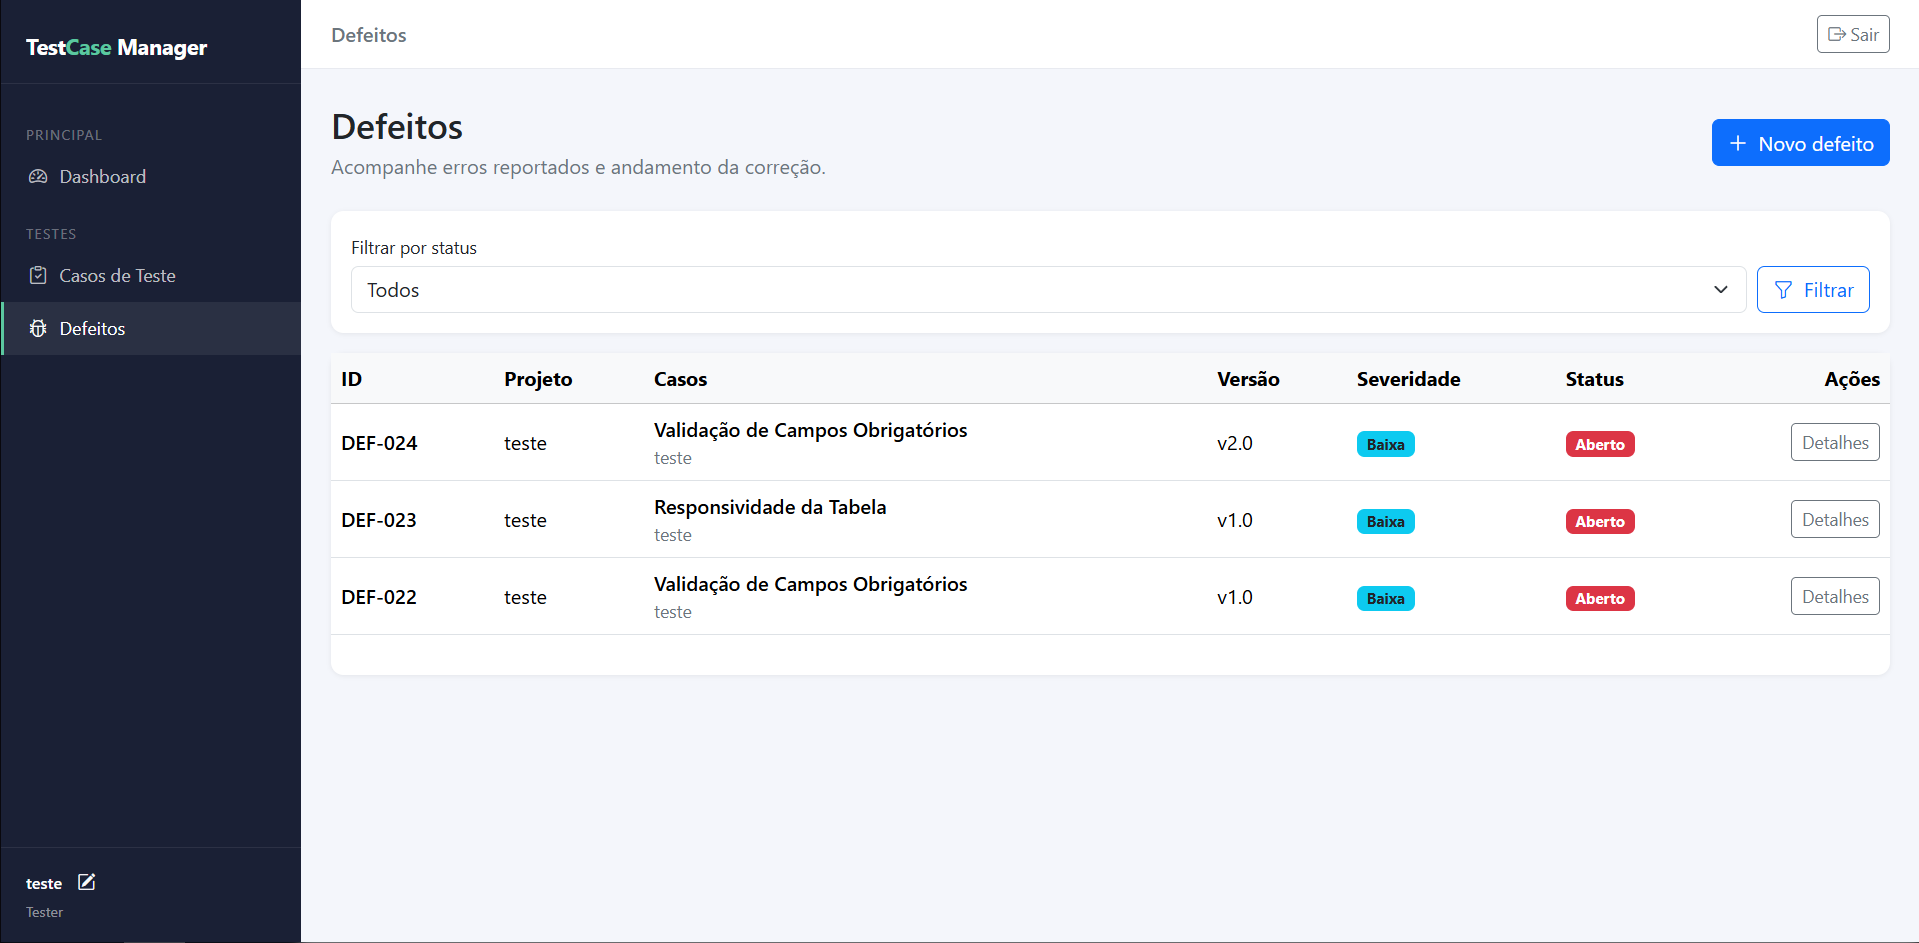
\includegraphics[width=0.92\textwidth, height=0.75\textheight, keepaspectratio]{./figuras/tela_defeitos.png} \\
    \vspace{0.2cm}
    {\raggedright \small Fonte: Elaborado pelo autor (2026).\par}
\end{figure}